\begin{frame}{Scatter Plot with Data Points}
\begin{center}
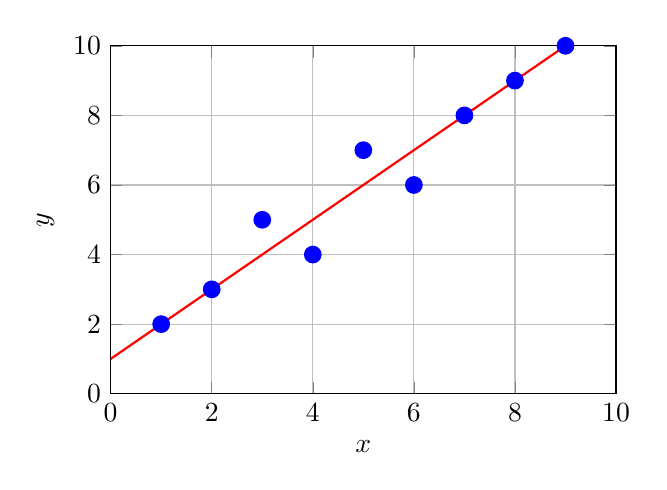
\begin{tikzpicture}
\begin{axis}[
    xlabel={$x$},
    ylabel={$y$},
    grid=both,
    xmin=0, xmax=10,
    ymin=0, ymax=10,
    width=8cm,
    height=6cm
]
\addplot[only marks, mark=*, mark size=3pt, blue] coordinates {
    (1,2) (2,3) (3,5) (4,4) (5,7) (6,6) (7,8) (8,9) (9,10)
};
\addplot[thick, red, domain=0:10] {x + 1};
\end{axis}
\end{tikzpicture}
\end{center}

\footnotesize
\texttt{\textbackslash addplot[only marks, mark=*, mark size=3pt, blue] coordinates \{\}}
\end{frame}